\documentclass[12pt]{article}
\usepackage{preamble}
\usepackage[hyperref=true,defernumbers=true,backend=biber,style=authoryear, citestyle=authoryear, firstinits=true, isbn=false, url=false, doi=false]{biblatex}
\addbibresource{reference.bib}
\title{Understanding User Incentives on Q\&A Sites:\\{\emph{An Analysis of Mathematics Stack Exchange Data}}}
% \subtitle{An Analysis of Mathematics Stack Exchange Data}
\author{Fei Li\footnote{Email: fei.li@studbocconi.it. This report is for the final project of the \emph{Business Analytics} course taught at Bocconi University. The code for producing this analysis is available on my \href{https://github.com/franli/business-analytics-project}{GitHub}.}}
\date{}
\begin{document}
\begin{titlepage}
\maketitle
\thispagestyle{empty}
\begin{abstract}
In this project, we develop a model for predicting user reputations on Mathematics Stack Exchange based on users' answer and question data. Our model is able to achieve nearly perfect performance for prediction. In our analysis we also highlight difficulties faced by many users who struggle to gain reputations. The model can be used to identify potential high-profile users among the pool of newly registered users, improve our understanding of the dynamics of mathematics Q\&A, and also help to develop potential new products and attract more users. 
\end{abstract}
\end{titlepage}

\tableofcontents
\clearpage

\section{Introduction}
Q\&A sites represent a significant proportion of information on the Internet.
Familiar examples are Quora, Stack Exchange, reddit, Yahoo!Answers, reviews on Amazon, and many other Q\&A forums dedicated to specific domains. A better understanding of the dynamics of the content generating process on those websites can help site owners to improve their services, design better mechanisms and attract more users, which can potentially benefit all the people across the Internet. Different mechanisms used in a Q\&A website can elicit different user incentives (\cite{jet} and \cite{yilingchen}) and this can affect the contents generated on the website.  On the empirical side, \cite{stackoverflow} developed a model to predict, for new questions asked on StackOverflow, whether their page views exceed certain level one year later. \cite{myopia} developed a model to predict whether or not an answer will be eventually accepted, using data from all the Stack Exchange communities. 

In this project we investigate the Mathematics Stack Exchange website, the second largest community on the Stack Exchange network, after StackOverflow. We develop a model to predict, given all of a user's data on this website except anything that is directly related to reputations (e.g. reputations, the score for each answer), whether his or her reputation is among the top $1\%$ percent. Our contributions are two-fold. First, we choose to study question and answering of \emph{mathematics}, instead of general Q\&A. Mathematics is very different from other subjects. To answer a mathematical question, one has to first use his/her mathematical knowledge to perform reasoning, and there is no absolute guarantee that one can solve any mathematical problem proposed in a short period of time. One may have to write down a proof in a logical way, or do some calculations, or come up with some intuitive examples. Writing mathematical expressions can also be time-consuming. Answering mathematical questions is risky yet costly. It is thus interesting to see how users interact to exchange information about mathematics. Second, instead of analyzing questions or answers, we choose to analyze user profiles. This can provide us with a better understanding of user behaviors, and ultimately may provide the site owners with hints about how to improve the website. The rest of the report is organized as follows: In \cref{sec:data} we describe the data and do some exploratory data analysis. Then in \cref{sec:task} we formulate our prediction problem and do feature selection. We then train our model and then measure the performance of our model. \cref{implication} discusses implications of our analysis. Finally in \cref{sec:conclusion} we draw our conclusions and point out possible directions for future research.

% but the tables that are relevant in our analysis are: 
% \lstinline!Users.xml!, which consits of records of each users' reputation
% \lstinline!Posts.xml!, which consis
% \lstinline!Badges.xml!
\section{Dataset Description}\label{sec:data}
The full data (\textasciitilde10GB) of this website is downloaded from \href{https://data.stackexchange.com/help}{Stack Exchange Data Explorer}, the official interface for downloading and querying Stack Exchange data. The downloaded data consists of 8 \lstinline!xml! tables: \lstinline!Users.xml! and \lstinline!Posts.xml! etc. We parsed the data into several \lstinline!.csv! tables using Python's BeautifulSoup package as well as \href{https://en.wikipedia.org/wiki/Regular_expression}{regular expression}. \cref{website-stats} contains some basic statistics of the website. We see that there are more than 450K users on the Mathematics Stack Exchange website. More than 1 million questions and 1.4 million answers have been posted, and a total of 8 million votes have been casted, and 1 million badges have been awarded. 
\begin{table}
\centering
\begin{tabu} to 0.7\textwidth{X[l] X[r]}
\toprule
Users & 465K\\
Questions & 1M\\
Answers & 1.4M\\
Votes & 8M\\
Badges & 1M\\
\bottomrule
\end{tabu}
\caption{Statistics of \href{http://math.stackexchange.com/}{Mathematics Stack Exchange}}
\label{website-stats}
\end{table}
Since we are interested in predicting user reputations, let's take a look at the distribution of user reputations. As we can see from \cref{reputation}, the distribution of reputations is however extremely unbalanced: most of the total amount of reputations are concentrated in a small number of users. Nearly 50 percent of all the users are ``inactive'', meaning that they haven't answered, or asked any question since they created their accounts and they also do not have any other activities. 
\begin{figure}
\centering
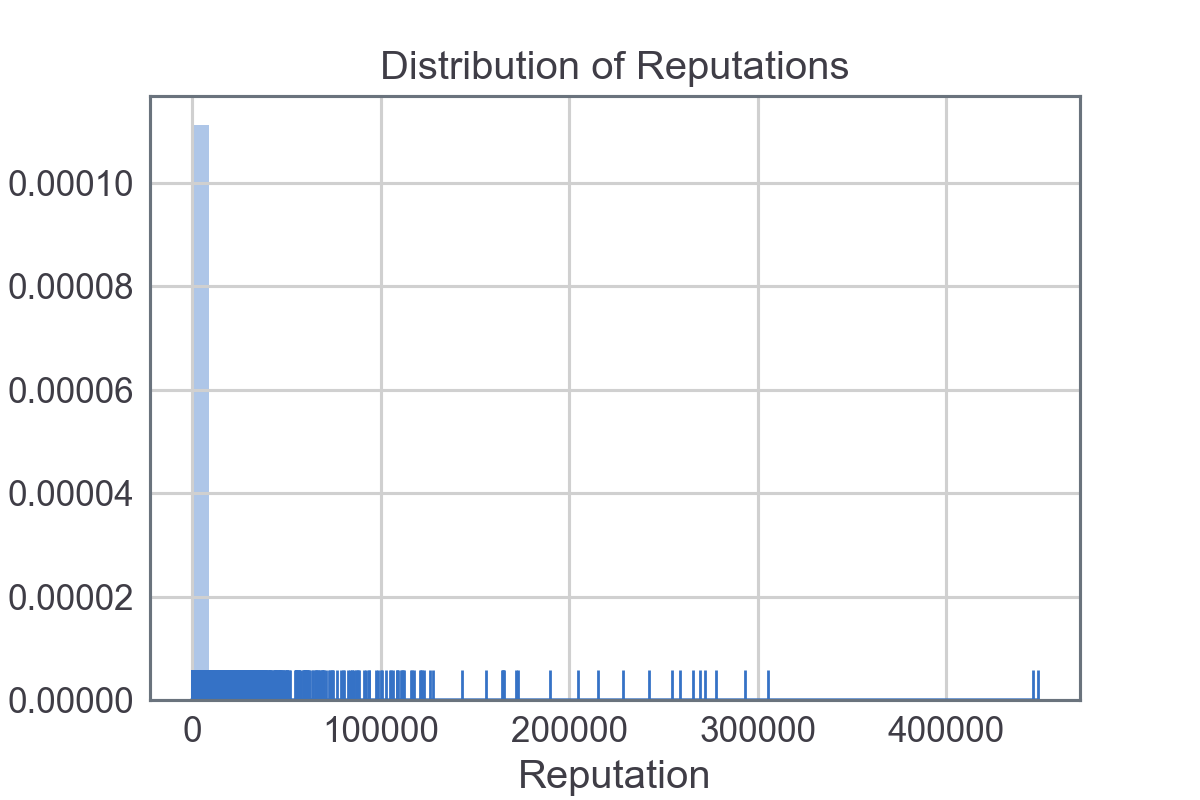
\includegraphics[width=0.8\textwidth]{figures/reputation_distribution.png}
\caption{Distribution of reputations. Small rugs represent individual observations.}
\label{reputation}
\end{figure}

Here are some individual data points: The top-one user is \href{https://math.stackexchange.com/users/12042/brian-m-scott}{Brian M. Scott}, an emeritus math professor in the United States, who has 450K reputations. As this article is written, he has 13,847 answers and he asked 0 question. Another interesting user is \href{https://math.stackexchange.com/users/97378/cleo}{Cleo}\footnote{On her profile page it states that ``\emph{My real name is Cleo, I'm female. I have a medical condition that makes it very difficult for me to engage in conversations, or post long answers, sorry for that. I like math and do my best to be useful at this site, although I realize my answers might be not useful for everyone}.'' Many people believe this is a fake statement.},  who is good at solving crazy integration problems. She has answered 38 questions, asked 2 questions, and has 12,811 reputations.

Since vote casts are directly related to reputations\footnote{The exact rule is described on the \href{https://math.stackexchange.com/help/whats-reputation}{website}.}, let's have a look at the votes ever casted since the creation of the website\footnote{We have omitted several other vote types here, like ``close'', ``reopen'' and ``undeletion'', since they represent only a minor proportions and are not relevant to our current discussion.}:
\begin{table}
\centering
\begin{tabu} to 0.7\textwidth{X[l] X[r]}
\toprule
Upvotes & 68.5\%\\
Downvotes & 8.2\%\\
Answer Accepted & 6.6\%\\ 
\bottomrule
\end{tabu}
\caption{Statistics of votes}
\label{votes}
\end{table}

From \cref{votes}, the majority of votes casted are upvotes, and downvotes are relatively rare. Next we calculated, on average, the percentage of all the upvotes an answer received as a function of time. As we can see from \cref{average-vote-time}, when you post an answer, you expect to see 60\% of all the upvotes your answer would receive to arrive in the first 24 hours. This may help you predict the potential upvotes you can earn from posting this answer, based on the upvotes you received in the first 24 hours. Of course for many answers, upvotes gradually come, even after years since those answers were posted, but for the majority of the answers on the website the voting activity would diminish quickly after the first day.
\begin{figure}
\centering
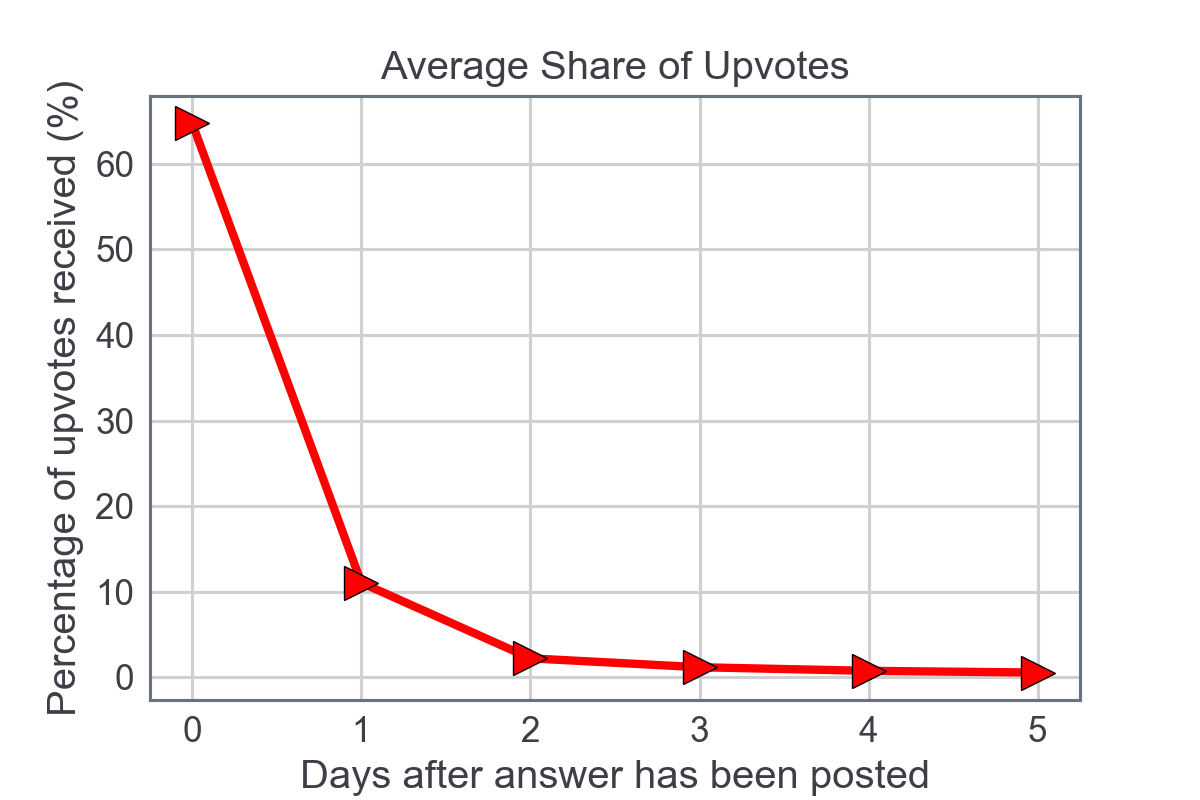
\includegraphics[width=0.8\textwidth]{figures/average-upvotes.png}
\caption{Average share of upvotes for answers as a function of time}
\label{average-vote-time}
\end{figure}

\section{Prediction Task}\label{sec:task}
Remember that our goal is to predict user reputations based on answer and question data. Specifically, the prediction problem is: \emph{given a user's answers and questions on this website, can we tell whether his/her reputation is among the top 1\%?} We calculated the top 1\% level reputation, and label an user as 1 if his/her reputation exceeds that level, and 0 otherwise. The task is to predict this label. We formulate the problem as a binary prediction task and we build a logistic regression model for doing the prediction. The reason for doing so is that there is a large dichotomy in terms of reputations: as \cref{reputation} has shown, some users have extremely high reputations and many do not. It is thus interesting to model this phenomenon and see what factors separate this two group of users. Using a linear regression for predicting reputations would put too much emphasis on predicting the exact numerical number, which is of less importance than the \emph{relative rank} of one's reputation among all (active) users. 

\subsection{Feature Selection}
From the data of answers and questions, how can we infer a user's reputation? Below we post some reasonings in selecting our features for predicting user reputations. Our selection of features is not purely for the purpose of prediction. Some features are included because they play important rules in shaping user's answering strategies, so we'd like to have an investigation of their effects. 

\emph{Does this user post a lot of answers?}~~The total number of answers is a natural predictor that one can think of: the more answers he/she give, the more reputations he/she may earn. From \cref{votes}, most of the votes on this website are upvotes, so when one posts an answer one generally expects to see more upvotes than downvotes. It is unlikely that a user will have a large number of answers with negative scores: since answering questions is costly, he/she does not have an incentive to continue to answer questions or even participate in this community if he/she gets a lot of downvotes. So if we see a user answers a lot of questions, then we should expect that those posts all have a positive contribution to the user's reputation. Thus the number of answers should be a strong indicator of user's reputation.

\emph{Does this user ask a lot of questions?}~~When you ask questions and people vote for your questions, you can also gain reputations. We thus also include the number of questions as a feature.

\emph{Does this user only answer OPs with high reputations, or he/she doesn't care about askers' reputations and answer questions asked by all levels of users?}~~Many new users are less experienced and are unfamiliar with the rules of the community. Many of the questions posted by new users do not meet the standard of the community and so are subject to further edits. Those users may not actively participate in the discussion after they post their questions, and they may not eventually accept answers. The proportion of people with relatively little mathematical maturity is also greater in the pool of new users than in users with some reputations. They may also not be able to judge the quality of the answers, and even if they finally accept answers, they may choose to accept an answer that is not the best one. For these reasons, overtime, people become less willing to answer their questions: your answer is less respected and the expectation of reputation gain is lower. In contrast, users with a certain accumulated level of reputation is more ``reliable''. The original poster (OP)'s reputation serves as a signal that he/she has been participating in this community, either by answering other people's questions or asking questions that are useful to others. They have high respect to answerers and are more likely to accept an answer. Thus, choosing to answer only questions asked by high reputation users may give your more reliable and steady gain of reputations. We thus calculated, for each user, the average reputation of OP he/she answered from the user's posts, and include this as a feature. 

\emph{Does the user usually post long answers or short answers?}~~People are easily attracted to long answers. An answer that occupies a great amount of space leave people with an impression that the answerer knows a lot, and has spent lots of time and energy in answering the question, \emph{even if its actual quality is lower than some shorter answers}. We calculated the average length of a post for each user and included this as a feature. Long answers are not necessarily good to the community. What really matters is the \emph{quality} of the answers. If people vote for answers according to their \emph{length} instead of \emph{quality}, then this may discourage high quality contributions and can lower the overall quality of the contents on the website.

\emph{How much mathematics vs. verbal explanations the user likes to use?}~~The Mathematics Stack Exchange website is where people ask and answer \emph{mathematics} questions, so we are interested in seeing whether people prefer more explanations in English or prefer more mathematical derivations. For each answer of each user, we divide the length of mathematical symbols used in that answer by the total length of the answer, to get the ratio of mathematical symbols for that answer. This indicates the proportion of mathematical expressions used in the answer. We then average across all the answers a user has, to get the average ratio for that user.

\emph{How quick does the user respond to new questions?}~~The data include, for each post (answer or question), its creation date, its poster, and its parent (for an answer this is the corresponding question and for a question this field is empty). We linked each answer to its corresponding question, subtracted the creation date of the answer by the creation date of the question, to get the response delay of this answer. Then for each user we averaged the response delay for all his/her answers and we use this as a feature in our model. The rationale is that the quicker you respond, the more attention you will get from the asker and other people, since new questions are displayed in the main page. In contrast, if you answered a question that was posted a long time ago, then few people will notice your answer and the asker may no longer use the website anymore, so you get fewer attention and thus fewer upvotes. We summarize our selected features in \cref{feature-table}.

\begin{table}
\centering
\renewcommand{\arraystretch}{1.5}
\begin{tabu} to \textwidth {X[l] X[1.5l]}
\toprule
\lstinline!Answer_Counts!& The number of answers that a user has\\
\lstinline!Question_Counts!& The number of questions that a user has\\
\lstinline!Average_OP_Reputation!& The average reputation of OPs that he or she answered\\
\lstinline!Average_Post_Length!& The average string length of the user's posts\\
\lstinline!Average_Math_Ratio!& The average proportion of mathematical symbols in a post\\
\lstinline!response_time!& The average response time to questions \\
\bottomrule
\end{tabu}
\caption{Features used in training the model}
\label{feature-table}
\end{table}

We then train our model, first using the whole dataset. The result of our logistic regression is summarized in \cref{regression-table}. All the features are standardized. The \lstinline!top_user! variable is our target variable that we want to predict, which equals to 1 if the user's reputation is among the top 1\% and 0 otherwise. The final observations consists of 234,332 observations, nearly half of the number of all registered users on the website. Users that are dropped are those who never had any activity on this website: no answer and no question. As we can see from the regression table, our model is able to explain the dependent variable well, with a pseudo $R$ squared\footnote{McFadden’s pseudo $R^2$ is $1-\ln\hat{L}(M_{\mathrm{full}})/\ln\hat{L}(M_{\mathrm{null}})$, where $\hat{L}$ is the estimated likelihood.} of 0.8147. The signs of all the coefficients are as expected, except perhaps the coefficient of \lstinline!Average_Math_Ratio!, which is negative. See \cref{implication} for interpretation of the result.
\begin{table}
\centering
\begin{tabu} to \textwidth{X[1.5l] X[1.5l] X[1.5l] X[0.8l]}
\toprule
\textbf{Dep. Variable:}          &     top\_user     & \textbf{  No. Observations:  } &   234332    \\
\textbf{Model:}                  &      Logit       & \textbf{  Df Residuals:      } &   234325    \\
\textbf{Method:}                 &       MLE        & \textbf{  Df Model:          } &        6    \\
\textbf{Date:}                   & Thu, 29 Nov 2018 & \textbf{  Pseudo R-squ.:     } &   0.8147    \\
\textbf{Time:}                   &     11:09:48     & \textbf{  Log-Likelihood:    } &   -2433.9   \\
\textbf{converged:}              &       True       & \textbf{  LL-Null:           } &   -13135.   \\
\bottomrule
\end{tabu}
\begin{tabu} to \textwidth{X[2.5l] X[r] X[r] X[r] X[r] X[r] X[r]}
\toprule
                                 & \textbf{coef} & \textbf{std err} & \textbf{z} & \textbf{P$>$$|$z$|$} & \textbf{[0.025} & \textbf{0.975]}  \\
\midrule
\textbf{Intercept}               &      -7.6515  &        0.104     &   -73.533  &         0.000        &       -7.855    &       -7.448     \\
\textbf{Answer\_Counts}          &     910.2201  &       14.586     &    62.406  &         0.000        &      881.633    &      938.807     \\
\textbf{Question\_Counts}        &      22.2786  &        0.790     &    28.191  &         0.000        &       20.730    &       23.828     \\
\textbf{Average\_OP\_Reputation} &       6.8320  &        0.719     &     9.505  &         0.000        &        5.423    &        8.241     \\
\textbf{Average\_Post\_Length}   &       8.2164  &        0.893     &     9.203  &         0.000        &        6.466    &        9.966     \\
\textbf{Average\_Math\_Ratio}    &      \textcolor{red}{-1.0521}  &        0.504     &    -2.086  &         0.037        &       -2.041    &       -0.064     \\
\textbf{response\_time\_seconds} &       1.4022  &        0.138     &    10.185  &         0.000        &        1.132    &        1.672     \\
\bottomrule
\end{tabu}
\caption{Logit regression results}
\label{regression-table}
\end{table}

\subsection{Performance}
We measure the performance of our model using the receiver operating characteristic (ROC) curve. See \cref{appendix-roc} for more information. The model achieves a nearly perfect classification, as can be seen from \cref{roc-all}.
\begin{figure}
\centering
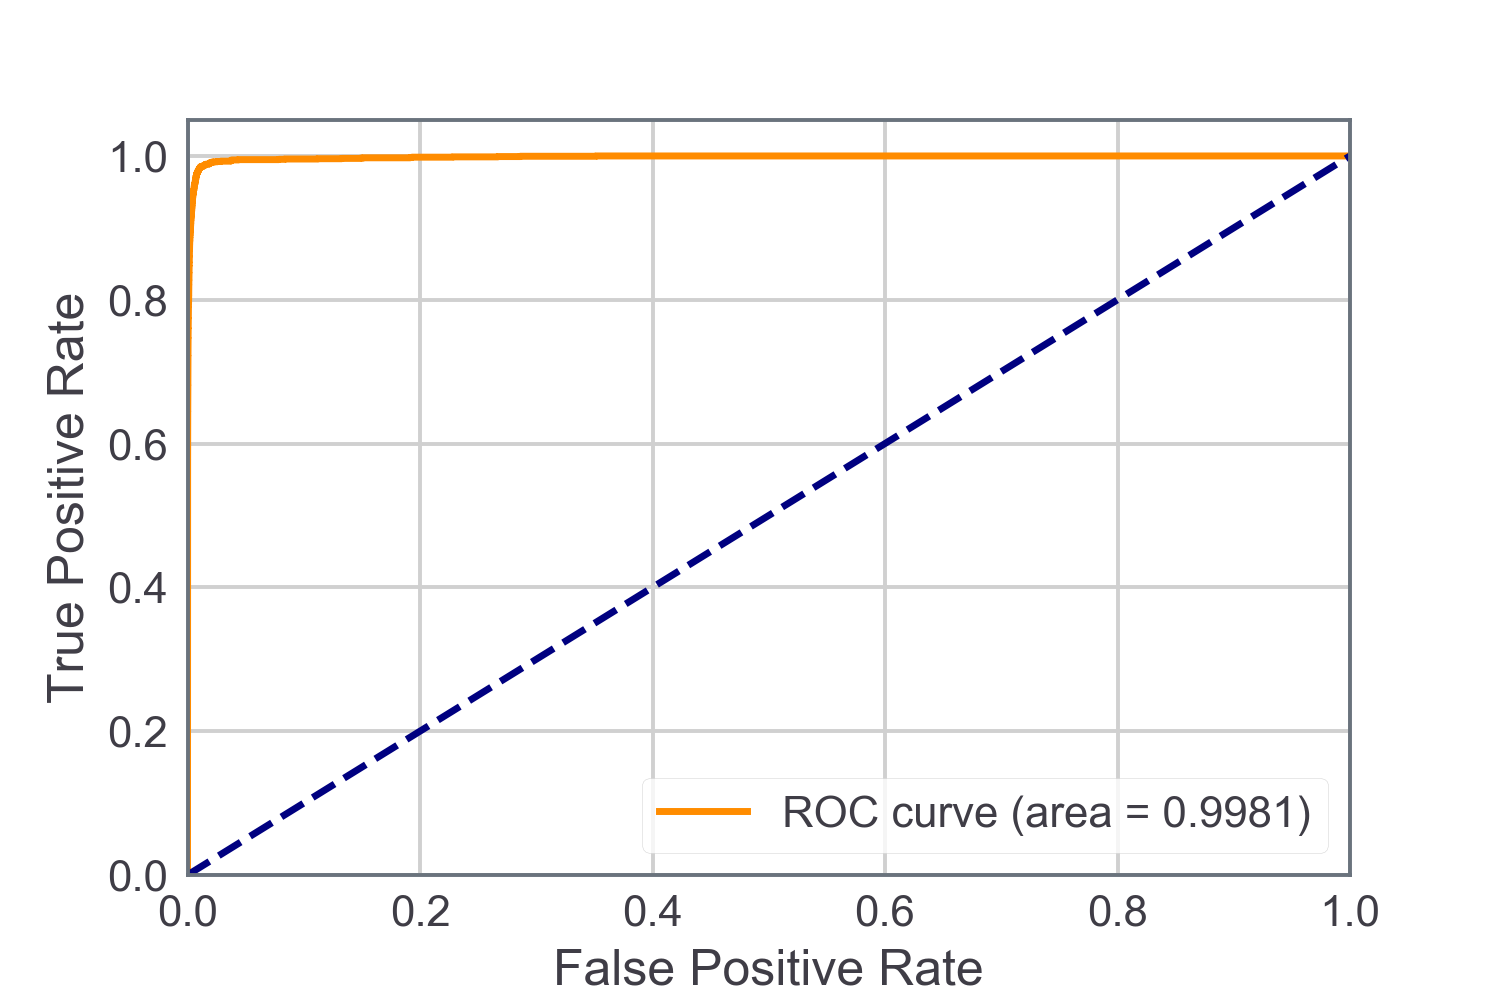
\includegraphics[width=0.69\textwidth]{figures/roc_standardized_features.png}
\caption{ROC curve of the model, trained using the whole dataset}
\label{roc-all}
\end{figure}
To address the issue of over-fitting, we performed 10 fold cross-validation. As we can see from \cref{10-fold}, our classifier is still able to achieve an AUC of 0.92 with 0.04 standard deviation. 
\begin{figure}
\centering
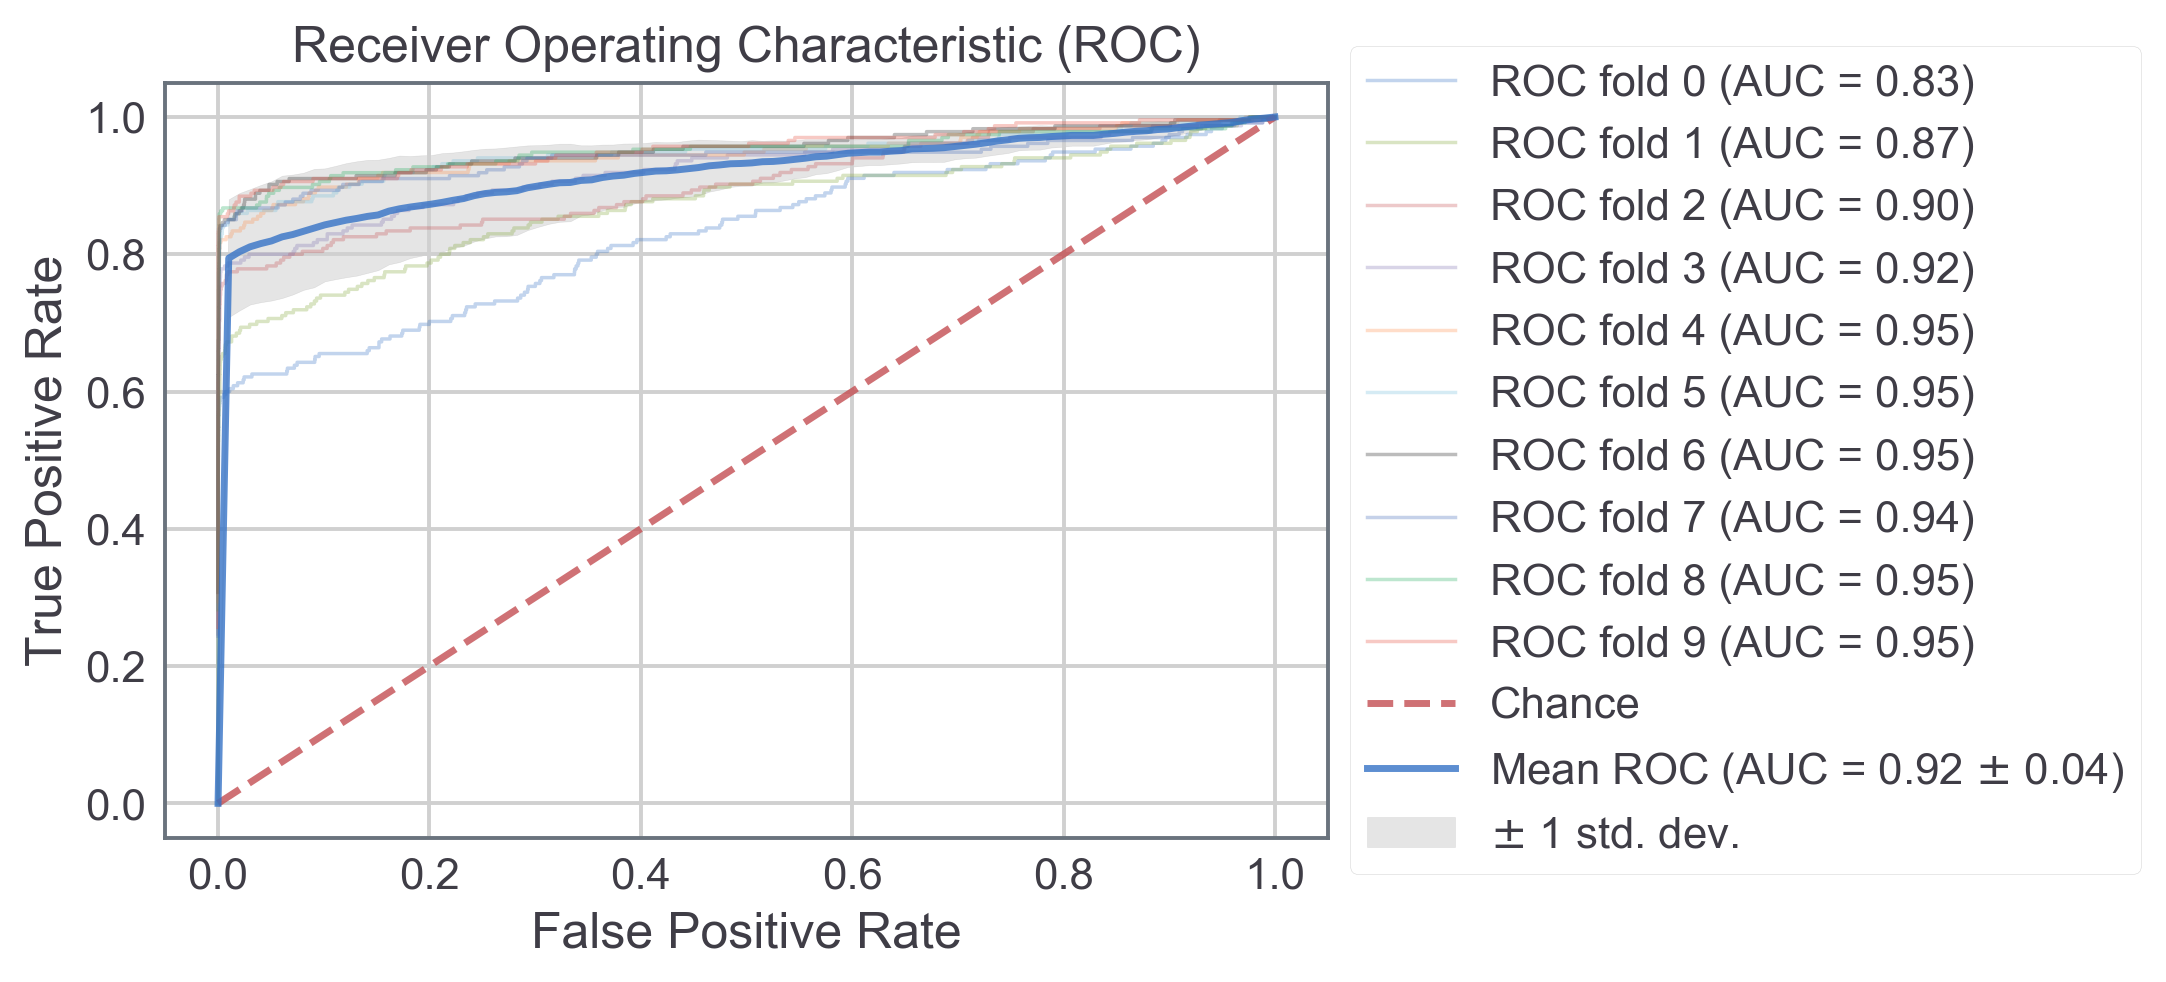
\includegraphics[width=\textwidth]{figures/roc-with-cv.png}
\caption{ROC curve with 10-fold cross-validation}
\label{10-fold}
\end{figure}

\section{Implications}
\label{implication}
% Let's now have a look at the regression table (\cref{regression-table}). 
\bi
\item Top users do not ask many questions. They are the ones that \emph{answer} a lot of questions. The pool of good questions is the core of the website. Since asking questions is less ``profitable'', the site should deliver more efforts in generating good questions. Many users become inactive after they registered on the website because they find that it is very difficult for them to answer questions. The website should make it easier for people to answer questions on the site.

\item We find that it is advantageous to answer questions posted by users with certain level of reputations, instead of those posted by new users. On the one hand, new users are often inexperienced and are unfamiliar with the rules of the community (e.g. they may not know that they should use \LaTeX~to type mathematical symbols). They are also not very likely to continue to stay in this community. Overtime people become less willing to answer their questions. To address the problem, the website has to make sure that new users get the instructions about how to make a post. They should also let old users be more friendly to new users. This is actually what we observed: the website now places a ``new contributor'' bar below icons of new users, to remind other people that this is a new user and they must follow proper code of conduct.

\item People with high reputations are those that stare at their computer screens all the time, wait for new questions and quickly respond. If you answer questions that were asked long time ago, then your answers are not likely to get much attention, and thus you will not gain much reputations in a short period of time. This is not good, since it implies that to earn reputation you have to spend a lot of time in front of your computer screen, which is demanding for most people. We predict that the site will provide incentives for users to answer old questions. And this is indeed the case. They have a badge called ``necromancer''\footnote{necromancy: the supposed practice of communicating with the dead, especially in order to predict the future.} which is awarded to answerers who answer a question more than 60 days later with a score of 5 or more. But we believe there are more that the site can do. For example, the website can display selected old questions on the front page. This can let users focus on answering questions, instead of chasing attention and votes.

\item If you use a lot of mathematics in your posts, then your chance of being a top user is smaller. This is consistent with what we observe: answers with high scores are those with more verbal explanations in them. It turns out that people like intuitions and explanations in plain English and they don't like to follow long derivations.
\ei

Under the current scheme, users have incentives to respond to only new questions, either by quickly writing and posting a long answer to draw attention, or by quickly posting some remarks, without necessarily going into the details and spending time and energy doing the calculations or proofs. Users do not have enough incentives to answer questions that were posted some times ago, even if those questions have not been sufficiently answered. Since only those quick or long answers are easy to get upvotes, scores of an answer (\#upvotes$-$\#downvotes) may not reflect the true quality of its content. 

In order to address the current issues and to attract more users, the website should encourage good question-asking practices. It should make it easier for users with all mathematical levels to answer questions on this website. Make sure that everyone can participate in this community. While the website operates on top of efficiency that was established through the reputation system, high level of inequality is not good for the long-run development of the website. A more equal mechanism should be designed to elicit more participation.


The model we developed has many possible applications. For example, it can be used to identify potential high-profile users from the pool of newly registered users. If a user exhibits those features in the model (answer a lot of questions, respond quickly to new questions, post long answers, use more verbal explanations etc.) then there is a large probability that this user will become a long-time contributor to this website. In contrast if a user becomes inactive not long after he/she registered, then it is likely that he/she will not continue to participate in this community. This gives the website more quantitative information about its users. The model can also be used to group users according to their preferences and make personalized recommendations, in order to increase participation and let more users get reputations in an easier way. It would also be useful if the website would like to develop new products, e.g. digests, feeds, periodicals etc. 

\section{Conclusion}\label{sec:conclusion}
In this project we analyzed user incentives on the Mathematics Stack Exchange website. We find that users with top reputations are those who: answer a lot of questions, especially questions asked by users with certain level of reputations; post answers that occupy a large space; use more English explanations rather than mathematical expressions; and quickly respond to newly asked questions. While competition for attention and upvotes among users can stimulate quick responses, which is a good thing for the askers, the \emph{quality} of the answers under the current incentive scheme may be inferior than if users were free from competing votes in a short time. Also, new users would find it hard to join this competition. To improve the quality of questions and answers, the website can have more interventions: select good questions and answers and feed them to users, so as to provide a guidance of generating high quality contents; make personalized recommendations for each user according to their preferences. Future research can continue to explore user interactions on the website. It would also be useful to experiment with alternative mechanisms for eliciting user-generated information.

\printbibliography
\clearpage

\section{Appendix}\label{appendix-roc}
In this section we provide an introduction to ROC curve and the area under the ROC curve (AUC), a commonly used metric in machine learning for measuring the performance of a binary classifier. Below I will use ``positive class and negative class'' with ``1 and 0'' interchangeably. First are some notations. Given a threshold $T$, a logistic regression classifier $\mathcal{F}$ maps each sample $y\in\{0,1\}$ to $\mathcal{F}(y)\in\{0,1\}$ by comparing the predicted score $\hat{y}\in[0,1]$ with the threshold $T$. If $\hat{y}\geq T$ then $\mathcal{F}(y)=1$ and if $\hat{y} < T$ then $\mathcal{F}(y)=0$. There are four cases:
\bi
\item If $y = \mathcal{F}(y) = 0$ then the sample $y$ is a \emph{true negative (TN)}.
\item If $y = \mathcal{F}(y) = 1$ then the sample $y$ is a \emph{true positive (TP)}.
\item If $y = 0, \mathcal{F}(y) = 1$ then the sample $y$ is a \emph{false positive (FP)}.
\item If $y = 1, \mathcal{F}(y) = 0$ then the sample $y$ is a \emph{false negative (FN)}.
\ei

A receiver operating characteristic (ROC) curve is a plot of \textbf{true positive rate (TPR)} against \textbf{false positive rate (FPR)} at various classification thresholds:
\bi
\item The true positive rate is how much the classifier gets it right among the positive samples. It is defined as the size of the true positives divided by the size of all positive samples, which consist of both true positives and false negatives.
 \[TPR = \frac{TP}{TP + FN}\]
\item The false positive rate is how much the classifier gets it wrong among the negative samples. It is defined as the size of the false positives divided by the size of all negative samples, which consist of both false positives and true negatives.
\[FPR = \frac{FP}{FP + TN}\]
\ei
\begin{figure}
\centering
\subfloat[perfect]{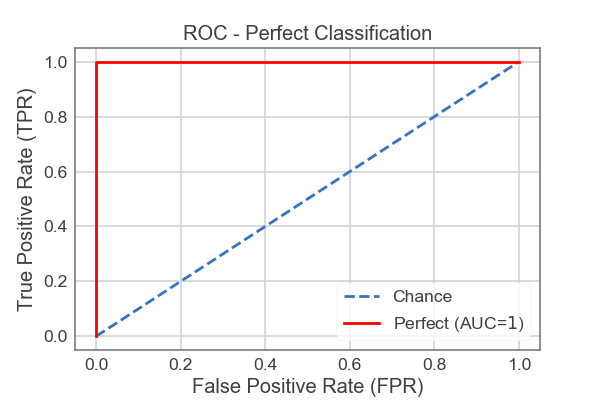
\includegraphics[width=0.5\textwidth]{figures/auc1.png}\label{subfig:perfect}}
\subfloat[reversed]{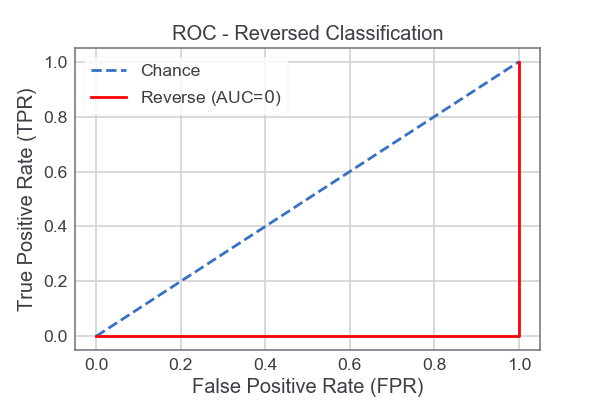
\includegraphics[width=0.5\textwidth]{figures/auc0.png} \label{subfig:reversed}}

\subfloat[random]{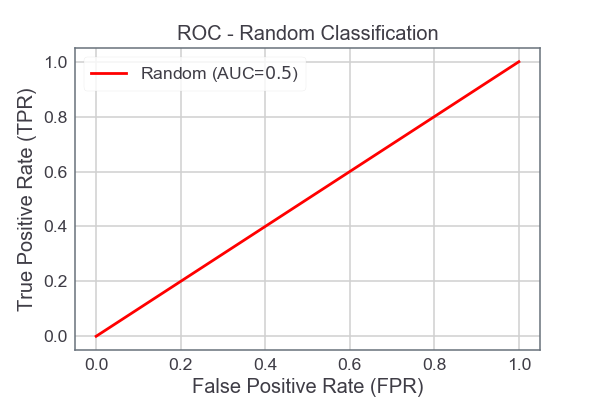
\includegraphics[width=0.5\textwidth]{figures/auc05.png}\label{subfig:random}}
\caption{ROC curves for three extreme cases}
\end{figure}
In general, the closer the ROC curve is to the upper left corner, the better. If the ROC curve passes point $(0,1)$, as in \cref{subfig:perfect}, it means that the classifier is able to achieve 100\% true positive rate and 0\% false positive rate, which implies that the model does perfect classification: it classifies every positive sample as positive and every negative sample as negative. If, on the other hand, the ROC curve is like \cref{subfig:reversed}, then the model classifies every positive sample as negative and every negative sample as positive. But this is actually not a bad thing: we just need to reverse the prediction for every sample and then we can get perfect classification. If the ROC curve is close to the 45\degree line, then it means that the model is no much better than randomly classifying some samples as positive and randomly classifying some samples as negative.

A natural metric for comparing ROC curve is the area under the ROC curve (AUC). $AUC=1$ corresponds to the perfect classification case, and $AUC=0$ corresponds to the reversed classification case. The closer the $AUC$ is to 1, the better. The area under the ROC curve (AUC) also has a probabilistic interpretation: \emph{It is the probability that the classifier ranks a randomly chosen positive sample higher than a randomly chosen negative sample.} Derivation of this probabilistic interpretation is as follows: let $S_1\in[0,1]$ denote the output score for a positive sample and let $f_1$ denote its density function. Similarly let $S_0\in[0,1]$ denote the output score for a negative sample and let $f_0$ denote its density. Let $\tau$ denote a threshold. The true positive rate as a function of the threshold is $\displaystyle tpr(\tau)=\mathbb{E}[S_1>\tau]=\int_{\tau}^1f_1$, and the false positive rate is $\displaystyle fpr(\tau)=\mathbb{E}[S_0>\tau]=\int_{\tau}^1f_0$. We have
\[\begin{split}
AUC &= \int_1^0tpr(\tau)d fpr(\tau) =\int_1^0 tpr(\tau)d\left(\int_{\tau}^1f_0\right)\\
 &=\int_0^1tpr(\tau)f_0(\tau)d\tau = \int_0^1\left(\int_{\tau}^1f_1\right)f_0(\tau)d\tau\\
 &= \int_0^1 \mathbb{E}[S_1>\tau]\cdot f_0(\tau)d\tau = \mathbb{E}[S_1>S_0]\\
 &= \mathbb{P}(S_1>S_0).\\
\end{split}\]


% \begin{figure}
% \centering
% \begin{minipage}{\textwidth}
% 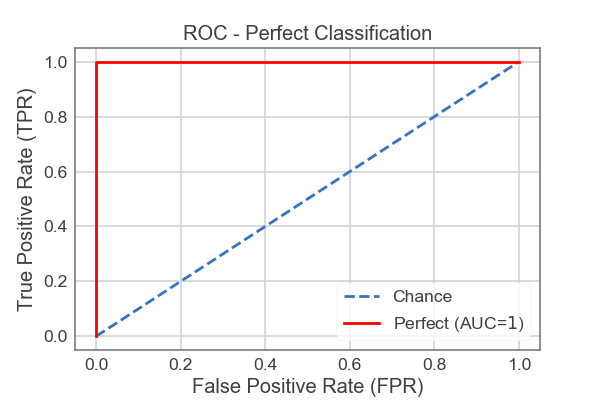
\includegraphics[width=0.5\columnwidth]{figures/auc1.png}  
% 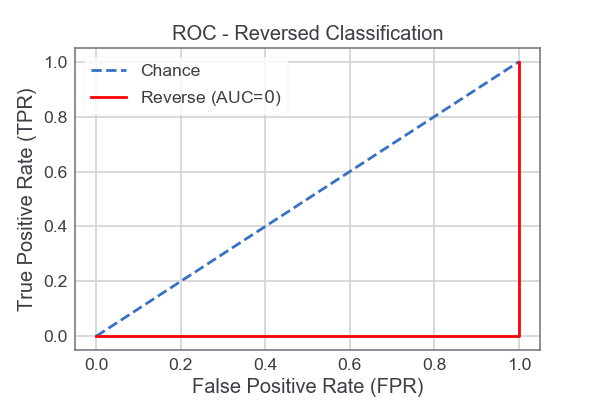
\includegraphics[width=0.5\columnwidth]{figures/auc0.png} 
% \end{minipage}
% \begin{minipage}{0.8\textwidth}
% 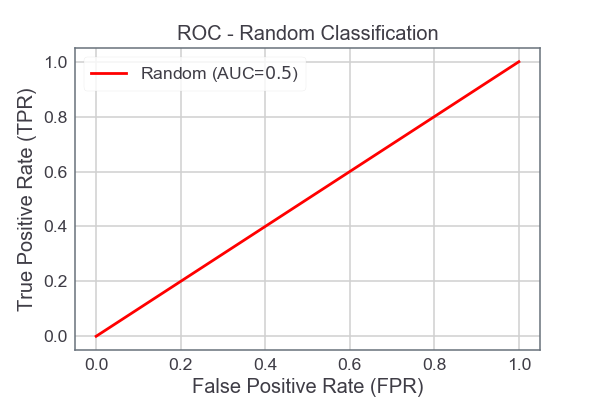
\includegraphics[width=0.5\textwidth]{figures/auc05.png}
% \end{minipage}
% \caption{ROC curves for three extreme cases}
% \end{figure}



\end{document}